\documentclass[12pt]{article}
\usepackage[utf8]{inputenc}
\usepackage{graphicx}
\graphicspath{ {./images/} }

\renewcommand{\baselinestretch}{1.5}
\title{La Jerarquía de Chomsky.}
\author{Luis Diego Jiménez Delgado\\ 2CM5}
\date{24 de septiembre del 2019}

\begin{document}

\maketitle

\textbf{La Jerarquía de Chomsky.} \\
La jerarquía de Chomsky es aquella que se usa para tener un sistema jerárquico de para clasificar  de manera matemática los lenguajes formales en 4 categorías, para también incluir sus formalizadores de cada lenguaje y también sus generadores y autómata de los mismos para reconocer a cada uno de ellos. 
\\ Sea un lenguaje L definido por al menos una gramática G que cumple:
\\
    \begin{itemize}
        \item Si todas las producciones de G tienen la forma ó donde A y B son simbolos no terminales y x es un terminal; entonces G se dice que es una gramática regular y L es un lenguaje regular o de tipo 3.
        \item Si todas las producciones de G tienen la forma donde x es una combinación de símbolos terminales y no terminales, entonces G se dice que es una gramática libre de contexto y L es un lenguaje libre de contexto o de tipo 2.
        \item De ser las producciones de G de la forma donde A es un símbolo no terminal cualquiera, x, y, y z son combinaciones de terminales y no terminales, tales que x e y pueden ser cadenas vacías; entonces se dice que G es una gramática dependiente del contexto y L es un lenguaje dependiente del contexto o lenguaje de tipo 1.
        \item Si ninguna de las gramáticas de L cumple las propiedades anteriores entonces se dice que es un lenguaje sin restricciones, recursivamente enumerable o de tipo 0.
        \item Genera un archivo para visualizar los resultados.
    \end{itemize}
Se añade el diagrama de la clasificación:\\
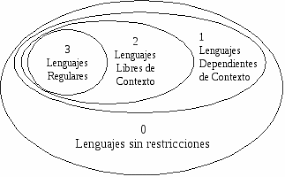
\includegraphics{Unknown}
\end{document}